\documentclass{article} 
\usepackage{geometry,amssymb,amsmath,listings,graphicx,xcolor,float,cancel}
\usepackage{tikz}
\usetikzlibrary{shapes,arrows}
\geometry{
	a4paper,
	total={170mm,257mm},
	left=20mm,
	top=20mm,
}

\lstdefinestyle{base}{
	language=Python,
	emptylines=1,
	breaklines=true,
	basicstyle=\ttfamily\color{black},
	moredelim=**[is][\color{red}]{@}{@},
}

\linespread{1.5}
\title{Map Anything Challenge Discussion}

\author{
  D'Azevedo, Gloria\\
  \texttt{gloria.dazevedo@gmail.com}\\
}
\date{May 2018}

\begin{document}
\maketitle

\section{Question 1: Create an distance matrix for a set of locations using only a list of latitudes and longitude pairs}
\subsection{Approach 1: List Solution}
The idea of using this solution was such to preserve the order of the locations (only denoted by a latitude and longitude without a unique identifier) and then create an distance matrix for distances between points i and j.  This solution when implemented correctly would save about half of the storage space to be on the magnitude of $\frac{n^2-n}{2}$ instead of $n^2$.Assuming the distance between two points are the same, no matter the direction, we only need to construct
the upper right half of the matrix denoted $x_{ij}, j>i$.  Also note that the diagonal would always be 0 since a point is always 0 distance from itself and we would not need to store it.  I have implemented a ``list of lists" solution where the wrapping list denotes the row number while the second index is a function of both the row number and the location number.  \\

There are limitations to this approach.  To access the distances between two points, the user would first have to know the order of the locations in the input file which would not necessarily be the easiest to go through.  The current assumed implementation does not have a key or location identifier which could potentially make that lookup easier as well.  In addition, due to the construction of the list of lists, the length of each sublist decreases as the rows increase.  Thus, to access $A[i,j]$ as expected in mathematical notation, the actual lookup would look more like $A[i][(j-1)-i]$ assuming that $i<j$

\subsection{Approach 2: Dictionary Solution V1}
This idea improves from the first approach of requiring the knowledge of the order of the locations and their indices in the original list.  The major differences between this approach and Approach 1 is that instead of storing the distance matrix as a list of lists, we create one tuple for each possible combination of location pairs. \\

When accessing the dictionary (done in $O(1)$) the code is easier to interpret since the actual latitudes and longitudes are used to access the values in the dictionary.  However, since this version of the implementation uses a tuple to denote a pair of locations, only one (ordered) copy of the pair is stored as key.  As an example, we would store the distance between $A$ and $B$ as $dict[(A,B)]$.  However, if we called $dict[(B,A)]$ then no such key would exist.  Thus we would need to know the specific order of the locations in the tuple to access that distance. 

\subsection{Approach 3: Dictionary Solution V2}
This approach is essentially the same as the Dictionary Solution V1 except instead of adding just one tuple to the dictionary as a key, we add both ``versions" of the latitude and longitude order as tuples in the dictionary.  To illustrate, we would add both $(A,B)$ and $(B,A)$ to the dictionary keys.  In this method, to access the distance is still $O(1)$ time but the amount of storage would essentially double from Approach 2.\\

If there was some previously defined location pair convention method such as the location with the lowest value of latitude goes first in the tuple for accessing and storing the dictionary key, then this solution would satisfy both the storage problem and the location pair access problem!

\section{Question 2: Find a Solution for the Schedule}
\textbf{Goal:} Need to minimize the number of drivers such that all clients are
(mostly) satisfied, we can make all deliveries within the week and other constraints
such as client service time and travel time are reasonable (full list in problem specifications).\\

\tikzstyle{block} = [rectangle, draw, 
text width=50em, text centered, rounded corners, minimum height=4em]
\tikzstyle{line} = [draw, -latex']
\begin{tikzpicture}[node distance = 7em, auto]
	\centering
	%blocks
	\node [block] (init) {Step 1: Assign location delivery day of week based on historical data to be a constraint};
	\node [block, below of=init] (identify) {Step 2: For each day of week, find the maximum distance or trip duration between any two locations with scheduled deliveries on that day};
	\node [block, below of=identify] (personbound) {Step 3: Determine upper bound of salesperson requirements to make all deliveries using maximum travel time and expected appointment time};
	\node [block, below of=personbound] (jobassignment) {Step 4: Use hierarchical clustering to cluster locations by distance or travel time then form $n$ clusters representing the number of salespeople required};
	\node [block, below of=jobassignment] (scheduling) {Step 5: For each cluster of locations that a salesperson would need to visit, we need to solve the travelling salesman problem for each location set};
	
	%lines connecting to the blocks
	\path [line] (init) -- (identify);
	\path [line] (identify) -- (personbound);
	\path [line] (personbound) -- (jobassignment);
	\path [line] (jobassignment) -- (scheduling);
\end{tikzpicture}


The following sections will discuss possible approaches and assumptions to find feasible solutions and how to improve them.

\subsection{Add Constraints: Deliver to each customer on their preferred date}
One of the ways we can create a schedule is to assume that each person does not have to work each weekday.  Instead we staff each weekday separately (i.e. Monday can have a different number of salespeople working than Tuesday) and guarantee that each customer has their deliveries on the preferred date (based on the past data).\\  

In business context, we want to appease our customers so barring unexpected emergencies, we plan to deliver on their preferred date.  Since the demand may not be equal for each day, then some salespeople will not work all 5 days of the week but that could free up some capacity to take new customers, adjusting schedules if something goes wrong, or they prefer to work part time.  In addition, even though it may not be optimal, by setting the number of deliveries by day to be constraints, it's one less variable to compute in the overall solution so we could potentially find a solution with uneven people working per day then manually adjust for a specific day of week.\\

\subsection{Determine upper and lower bound for salespeople per day}
Once the set of customers per day are determined, we can create bounds for the number of salespeople required per weekday.  Since we have the set of locations that we need to service, we can create the distance matrix for that set of locations similar to the earlier problem.  Then, we know how long each appointment will take (20 minutes) and a max time that it would take between two locations in the set.\\

Similar to the distance matrix calculation, we can extract the time it takes between two locations instead of physical distance.  If we call this maximum time $T$ then the minimum number of trips a salesperson can take is solved by $max_n: 480 \geq 20n+T(n-1)$ for an integer $n$ since there are only 8 hours in a day (480 minutes) for them to work and they would need to make $n-1$ transitions between the $n$ stops with the assumptions that they start and end exactly at 9 am and 5 pm.\\

Similarly, to find the maximum number of stops they can make in a day where $t$ is the minimum time between two points in this set of locations is such that $max_m:480\geq 20m+t(m-1)$ for an integer $m$ where the additional assumption is that $t\leq T$.  Both of these assumptions assume no extra time built in for transitioning between the sale appointment and the travel time (like getting in the car or a lunch break). This extra time could be built in by decreasing the ``max time" in a day from 480 minutes to say 450 minutes with the assumption that breaks can be taken anywhere and at any point.\\

To find a bound for the number of people required, we would divide the total demand $D$ for that day by the bounds for the jobs per person.  The lower bound is computed as $L=\lceil\frac{D}{m}\rceil$ while the upper bound is computed as $U=\lceil\frac{D}{n}\rceil$.  For illustration, assume that the upper bound $U$ of expected salespeople are used to guarantee a solution.\\

\subsection{Assigning locations to salespeople for a day's demanded delivery}
So at this point in the procedure, for a certain weekday we know which locations are getting visited and how many people we need to allocate for that day.  We can use the distance matrix for this set of locations and use a clustering technique based on the distance or time between locations to determine which ones are closest to each other.  Once we create this set and look at the dendrogram, we can segment the set of locations into $U$ clusters of around $n$ locations each.  An example of cutting a dendrogram can be found below where the solid horizontal flat line corresponds to cutting the data into 3 mutually exclusive groups: \\

\begin{figure}[H]
	\centering
	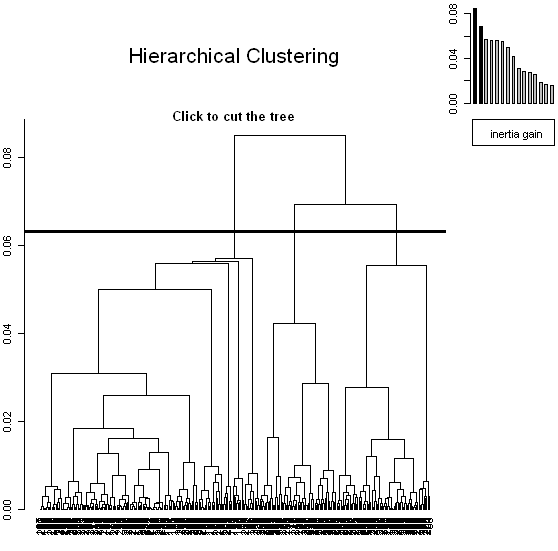
\includegraphics[scale=0.50]{hierarchical_clustering_example}
	\label{fig:Hierarchical Clustering Dendrogram Example}
\end{figure}

The distribution of locations from the dendrogram cut may not shake out to exactly $n$ locations per salesperson but since each location is at most $T$ distance away from another location, the locations can be reallocated to the next nearest salesperson clique so that they all work for the same amount of time per day.  Depending on client locations, for example, one person could see 8 clients that are close together while another could see 2 clients that are far apart.  If using a sales person estimate lower than $U$ then more adjustment would have to be done to assign locations to people.\\

\subsection{Schedule appointments (order of location visiting)}
In order to assign the order of locations that a salesperson visits, it's unsurprisingly a travelling salesman problem. Ha-ha. For the context of this problem, we note that there is at most $n$ stops to make so we could use brute force to calculate the possible permutations $n!$ of order of locations to get the order of locations with the minimum time. This method would guarantee the lowest distance but could easily be very computationally expensive even with slightly larger values of $n$.\\

Another way we could reduce computation time is to again do a clustering technique within the salesperson's locations using the distance.  However, instead of cutting the dendrogram to make clusters, we start at the bottom most node, then travel to the next closest location, then the next closest location from there and so on until all locations are completed.  By construction, each leg would be smaller than $T$ so there should be a feasible solution.\\

\subsection{Results and Solution Implications}
Once we have this conservative feasible solution, then what? One possible metric is how much excess time the solution yields, aggregated over all salespeople.  Excess time would be defined as the extra minutes in day that is not allocated to travelling or an appointment.  If a solution has high excess time then we may consider removing a salesperson and reallocating the customers to the remaining people.  The company itself may have benchmark KPIs with excess time greater than 0 to allocate for variations in travel, sickness, and unexpected occurrences so we can either build that into the model (see earlier remark about reducing maximum time from 480 minutes to a lower amount) or look at the excess time from the solution.\\

Another metric would be the amount of manual adjustment done to the solution (if any) between steps.  This metric is harder to measure but it would be calculated after the process is run and see if the solution is feasible or almost feasible.\\

Finally, there is inherently the tradeoff between computation time and solution optimality.  For this example it is possible that we could run all sorts of variable combinations but in real life that wouldn't be possible.  The run time of the solution generation combined with the excess time metric could be another KPI to benchmark against. Potentially we would want to increase computation power by a percent $p\%$ if it reduces the excess time by more than $p\%$ or some absolute amount.\\

\subsection{Further Optimization and Potential Decision Factors}
During this discussion, we assumed that we had unlimited potential resources (salespeople, no travel costs other than time, salary expense) and that each client was treated equally (equal revenue, same appointment length of 20 minues).  However, in reality, each client will have different requirements and will be of different sizes so those factors would affect sales and whether or not we should continue doing business with them.\\

One possible improvement onto the above process given limited salespeople time would be to segment customers based on sales or size and target the segment with the largest sales first before allocating remaining resources for smaller clients.  This would be similar to a discrete packing problem where we want to hold onto the most valuable resources first given limited space (and assume 20 minutes for each slot) so the value per unit is highest. This would theoretically ensure that largest customers are served first but fewer customers maybe served overall if the large customers are very far away from each other and lots of time is spent travelling.  A function of this additional travel time problem could be factored in to the 20 minute appointment time so that it can be properly indexed and compared to the smaller customers.\\

Another potential way to optimize limited sales resources is to again look at hierarchical clusters of all the possible locations first (instead of the locations for a given weekday) and then assign salespeople to those clusters.  Then within those clusters, they can determine which clients to visit using the packing problem principal (roughly sales per minute taking into account travel time).  Note that because of construction using distance, the travel times should be lower within each cluster.  In addition, these sales people could be assigned to each cluster that's close to their house to minimize pre work travel and post work travel.\\ 


\end{document}